\documentclass[crop,tikz,varwidth]{standalone}
%\documentclass{article}
\usepackage{tikz}
%\usepackage{tikz-3dplot}
%\usetikzlibrary{patterns,calc,decorations.pathmorphing,angles,quotes,external}
\usetikzlibrary{angles,quotes}
\usepackage{MyStandard}
%\usepackage{MyChem}
%\usepackage{tikz-3dplot}
\pgfdeclarelayer{background}
\pgfdeclarelayer{foreground}
\pgfsetlayers{background,main,foreground}  

\begin{document}
\newcommand\Odraw[1]{\shadedraw[shading=radial,outer color=red!90,inner color=red!30,draw=black] {(#1)} circle(.5cm);}
\newcommand\Hdraw[1]{\shadedraw[shading=radial,outer color=blue!90,inner color=blue!30,draw=black] {(#1)} circle(.4cm);}
\newcommand\anghoh{\enmat{\theta(\te{HOH})}}
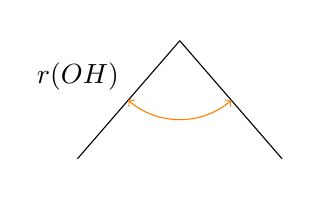
\begin{tikzpicture}
\begin{scope}
  \draw(1.3,1.5) node[circle,minimum size=.4] (O) {};
  \draw(0,0) node[circle,minimum size=.3] (H1) {};
  \draw(2.6,0) node[circle,minimum size=.3] (H2) {};
   \Odraw{O}
  \Hdraw{H1}
  \Hdraw{H2}
\begin{pgfonlayer}{background}
 \draw (O.center) -- node[above left]{$r(\te{OH})$} (H1.center);
 \draw (O.center) --  (H2.center);
 \draw pic["\anghoh", draw=orange, <->, angle eccentricity=1.2, angle radius=1.cm]
    {angle=H1--O--H2};
\end{pgfonlayer}
\end{scope}
\end{tikzpicture}
\end{document}